\chapter{Electrones identificados como fotones}\label{ch:e_fake}
\chaptermark{Electrones identificados como fotones}


Como ya se mencionó anteriormente, existe un fondo que contribuye a procesos asociados a fotones y jets como estado final, donde un electrón del estado final es identificado como un fotón. Este puede provenir de procesos del SM, como los que producen bosones $W$ y $Z$ + jets, y $\ttbar$. El mismo es difícil de estimar a partir de simulaciones, ya que dependen en gran medida de la estructura y material del detector que es muy compleja de modelar en todos sus detalles. El objetivo es entonces estimar este fondo calculando un factor de identificación errónea (\textit{Fake Factors}) en función de las variables $\eta$ y $p_{T}$ de los objetos a partir de los datos adquiridos.

\section{Medición del factor de identificación errónea}

El método para la estimación del factor de identificación errónea, hace uso de la muestra de eventos $Z\rightarrow ee$. En base a esta muestra, se determinan la relación de eventos de pares electrón-positrón y los paras electrón(positrón)-fotón cuya masa invariante es compatible con la del bosón $Z$. Estos últimos pares así seleccionados provienen de eventos en los cuales un electrón (positrón) del decaimiento del $Z$ es reconstruido como un fotón. El factor de identificación espuria se puede calcular entonces como: 

\begin{equation}
F_{e\rightarrow\gamma}[\eta , p_{T}]=\frac{N^{eg}[\eta , p_{T}]}{N^{ee}[\eta , p_{T}]} \label{eq:ff_ratio}
\end{equation}
\tosolve{definicion de Neg Nee?}

Como la muestra de pares de objetos seleccionada no es una muestra pura de $Z\rightarrow ee$, se realiza un ajuste a la distribución de su masa invariante para determinar por separado la contribución de señal y de fondo en cada muestra, como se explicará más adelante. \tosolve{no me gusta este parrafo aca}

Los criterios para seleccionar los objetos de los pares de partículas mencionados se explican a continuación y se basan en criterios de selección que mantengan una alta pureza de la muestra, manteniendo un bajo rechazo de señal.
Los electrones  son seleccionados con $p_{T} > 25 \egev$, con un criterio de calidad \textit{tight} y punto de trabajo de aislamiento denominado \textit{gradient loose} \cite{ATLAS-CONF-2016-024}. Para los fotones los requisitos son $p_{T} > 25 \egev$, \textit{tight} y aislados \cite{STDM-2010-08}. A ambos se les solicita que tengan un $\eta_{BE}<2.37$; que estén fuera de la región del \textit{crack} entre $1.37$ y $1.52$; que provengan del vértice primario en base a un parámetro de impacto $d_{0}$ con una significancia menor a 5, y que cumplan con la relación $|\Delta z_{0}\sin\theta|<5$.

Además, si un electrón y un fotón son reconstruidos con $\sqrt{\Delta\phi^{2}+\Delta\eta^{2}}<0.4$, el fotón es descartado del evento. Esto reduce precisamente la probabilidad de utilizar candidatos donde un electrón es reconstruido como fotón \tosolve{no usamos OR no?}. Para reducir la contaminación de fondo de $W (\rightarrow e\nu)$ se aplica finalmente un selección de eventos con $\met < 40 \egev$. 


A todos los pares se les solicita que una masa invariante entre $75$ y $105 \egev$  estando así en la región de cercanía a la masa del $Z$. Finalmente, en el caso de que existiese más de un par en el evento, se utiliza el que tiene la masa invariante más cercana a la del bosón $Z$ ($91.1876 \pm 0.0021 \egev$\cite{Olive:2016xmw}). Esto minimiza la contaminación de pares aleatorios, descartando solo unos pocos eventos donde pueda haber más de un $Z$ en estado final.


En base a los objetos seleccionados se crea un arreglo bidimensional en  $\eta$ y $p_{T}$. Para eventos positrón-electrón una entrada se realiza para cada partícula. En los casos de pares electrón-fotón un arreglo es creado por separado y los solo los valores de los fotones son utilizados.

La concepción del método proviene de la siguiente consideración. Sea $\epsilon_{i}$ la eficiencia de reconstruir un electrón, con un valor de $\eta$ y $p_{T}$ correspondientes al bin \textit{i} del histograma. Para una muestra de \textit{N} pares de electrones y positrones reales (dentro del rango de masa), decimos que $f_{ij}$ es la fracción de pares para los cuales el electrón \textit{leading} (\textit{sub-leading}) está dentro del bin \textit{i} (\textit{j}). Considerando solamente electrones-positrones provenientes del decaimiento de un bosón $Z$, el número de eventos en el bin \textit{i} del histograma $N^{ee}[\eta , p_{T}]$ es entonces:

\begin{equation}
N_{i}^{ee} = \sum_{i}\epsilon_{i}\epsilon_{j}f_{ij}N + \sum_{j}\epsilon_{j}\epsilon_{i}f_{ji}N = \epsilon_{i}N\sum_{j}\epsilon_{j}(f_{ij}+f_{ji})
\end{equation}

De forma análoga, ahora considerando que $p_{i}$ es la proporción de fotones reconstruidos como electrones en el bin \textit{i}, la cantidad de eventos en el bin \textit{i} del histograma $N^{eg}[\eta , p_{T}]$ es:

\begin{equation}
N_{i}^{eg} = \sum_{i}p_{i}\epsilon_{j}f_{ij}N + \sum_{j}p_{j}\epsilon_{i}f_{ji}N = p_{i}N\sum_{j}\epsilon_{j}(f_{ij}+f_{ji})
\end{equation}

El factor que determina la proporción de electrones reconstruidos como fotones se define finalmente como:

\begin{equation}
F_{e\rightarrow\gamma}[\eta , p_{T}]\equiv\frac{N^{eg}}{N^{ee}}=\frac{p_{i}}{\epsilon_{i}}
\end{equation}

Por ende, el factor, no es la proporción de fotones mal reconstruidos, sino que es el cociente entre esa proporción y la eficiencia de reconstruir un electrón. De esta forma el fondo correspondiente a electrones identificados como fotones resulta:

\begin{equation}
N_{e\rightarrow\gamma}(\eta , p_{T} , ... ) = F_{e\rightarrow\gamma}(\eta , p_{T})\cdot N_{e}(\eta , p_{T} , ...)
\end{equation}
	
Donde $N_{e}(\eta , p_{T} , ...)$ es el número de electrones en un determinado estado final correspondiente a las distintas regiones del estudio de partículas supersimétricas mencionado en el capítulo anterior. Estos eventos se seleccionan entonces requiriendo electrón en lugar de un fotón en el estado final. 

La implementación del cálculo en ROOT y C++ se  base en histogramas bidimensionales. Para cada evento que contiene un par electrón-positrón, en un histograma con bines de $\eta$ y $p_{T}$ ($N^{ee}[\eta , p_{T}]$), se suma una entrada en el bin correspondiente al $\eta$ y $p_{T}$ de cada uno de los electrones. En el caso de que el evento tenga un par electrón-fotón, en otro histograma ($N^{eg}[\eta , p_{T}]$), se suma una entrada en el bin correspondiente al $\eta$ y $p_{T}$, solamente del fotón. El correspondiente factor se obtiene entonces como en la ecuación \ref{eq:ff_ratio}.

Dado que los pares de objetos utilizados para el cálculo, tienen un probabilidad de no provenir del decaimiento del bosón $Z$, sino de otros procesos no resonantes de fondo, la relación entre señal y fondo tiene en cuenta en el calculo del factor buscado.
Para tener en cuenta la relación entre entradas correspondientes a la señal y las correspondientes al fondo, cada entrada en los histogramas es pesada con un peso representativo de esta relación.


\subsubsection{Clasificación de eventos}

La relación entre señal y fondo en la distribución de masa invariante de los eventos correspondientes a la masa del $Z$ se utiliza en el método para determinar un peso que se obtiene a su vez clasificando a los pares según el tipo ($ee/e\gamma$) y según la región donde se reconstruían los objetos \textit{endcap}-\textit{endcap} ($EE$), \textit{barrel}-\textit{endcap} ($BE$) y \textit{barrel}-\textit{barrel} ($BB$), ya que los factores de identificación erróneas dependen de la región del detector donde fueron reconstruidos dados los distinta morfología y tipo detectores utilizados en cada una ellas. Para cada una de las tres regiones se calcula su masa invariante de los pares, se realiza el correspondiente ajuste para determinar la contribución de señal (S) y fondo (B) y finalmente el peso resulta de la relación: $w=\frac{S}{S+B}$. 

Los datos utilizados para el análisis corresponden a los años 2015 y 2016 del Run 2 del LHC, en base a la denominada derivación EGAM1 que realiza una pre-selección de eventos optimizado para estudios del $Z$, con una base de electrones y fotones con $p_{T} > 15 \egev$ y masa invariante de los distintos tipos de pares mayor a 60 \egev. %y con ningún requisito de \textit{triggers}.

Para los ajustes de la masas invariantes se utiliza como modelo de señal una \textit{double-sided Crystall-ball} (DSCB). Para el fondo se utiliza un polinomio de grado 2. Los resultados de los ajustes obtenidos para cada clasificación de los pares se pueden observar en las Figuras \ref{fits_BB}, \ref{fits_BE} y \ref{fits_EE}.


En base a los resultados de estos ajustes se determina la contribución de señal y background en cada región, determinando así los correspondientes pesos como se mostrará en la sección \ref{sec:resultados} en la Tabla \label{ta:fftable} \tosolve{te refir a la tabla con pesos? podria ir la tabla con pesos, y no citarla en secciones futuras}.

Los electrones utilizados para estimar la contaminación de fotones de señal \textit{tight}, pueden pasar tanto requerimientos  \textit{medium} o \textit{tight}. En ambos casos se encuentra una buena relación señal y fondo, siendo naturalmente el caso de selección \textit{tight} la de mayor pureza a costa de una menor estadística de la muestra. Ambas selecciones se estudian en el presente trabajo como se discute en las siguientes secciones.


\subsection{Sistemáticos}

Las principales fuentes de incertezas sistemáticas del método para el calculo de los factores que determina la contaminación de fondo en las distintas regiones, proviene de las definiciones de las funciones y rangos de ajustes de los fits, así como de las ventanas de aceptación de pares.  Para estimar los posibles incertezas se varió el rango nominal de la masa de $[75-105]\egev$ a los rangos de $[70-110]\egev$ y a $[80-100]\egev$. Como caso extremo en la definición y criterios de ajuste, se determinaron los factores imponiendo los pesos $w=1$ eliminando así la sustracción de fondo en su cálculo. Los resultados de estos estudios se muestran el la Tabla \label{ta:fftable} donde se observa que la incerteza dominante proviene en base al criterio adoptado es la de tomar $w=1$ siendo esta del orden del $20 \%$ dominando sobre todo otra contribución.

\tosolve{mi propuesta para este parrafo:}

Las principales fuentes de incertezas sistemáticas del método para el calculo de los factores que determina la contaminación de fondo en las distintas regiones, proviene tanto de los ajustes a la masa invariante como de los criterios de aceptación de los pares.  Para estimar los posibles incertezas se varió el rango nominal de la masa de $[75-105]\egev$ a los rangos de $[70-110]\egev$ y a $[80-100]\egev$. Lo mismo se hizo con el rango del fit que se varió de su rango nominal $[70-110]\egev$, a $[65-115]\egev$ y a $[75-105]\egev$. 

Otro sistemático surgió de la utilización de una función diferente para modelar el fondo, en este caso se usó un polinomio de grado 3. Como caso extremo en la definición y criterios de ajuste, se determinaron los factores imponiendo los pesos $w=1$ eliminando así la sustracción de fondo en su cálculo. 

Los resultados de estos estudios se muestran el la Tabla \tosolve{tabla con syst} donde se observa que la incerteza dominante proviene en base al criterio adoptado es la de tomar $w=1$ siendo esta del orden del $20 \%$ dominando sobre todo otra contribución.


%Se consideran distintas fuentes de incertezas sistemáticas. Una de ellas proveniente de la variación tanto del rango del fit, como del rango de masa de aceptación de los pares. El rango nominal del fit es $[70-110]\egev$ y se varía a $[65-115]\egev$ y a $[75-105]\egev$. El rango nominal de la masa es $[75-105]\egev$ y se varía a $[70-110]\egev$ y a $[80-100]\egev$. Se tuvo en cuenta también como fuente de sistemático, la variación en los valores de los factores al utilizar otra función para el ajuste del fondo, utilizándose un polinomio de grado 3 y un polinomio de Bernstein de grado 4.


Los resultados obtenidos para el factor en bines de $\eta$ y $p_{T}$ se muestran en la Tabla \ref{ta:fftable} incluyendo por separada las incertezas estadísticas y sistemáticas del método (\tosolve{Agregar tabla de FF +stat + syst }).\tosolve{estos resultados (los FF) podrian ir en la siguiente seccion}




\begin{figure}

	\begin{subfigure}{0.5\textwidth}
		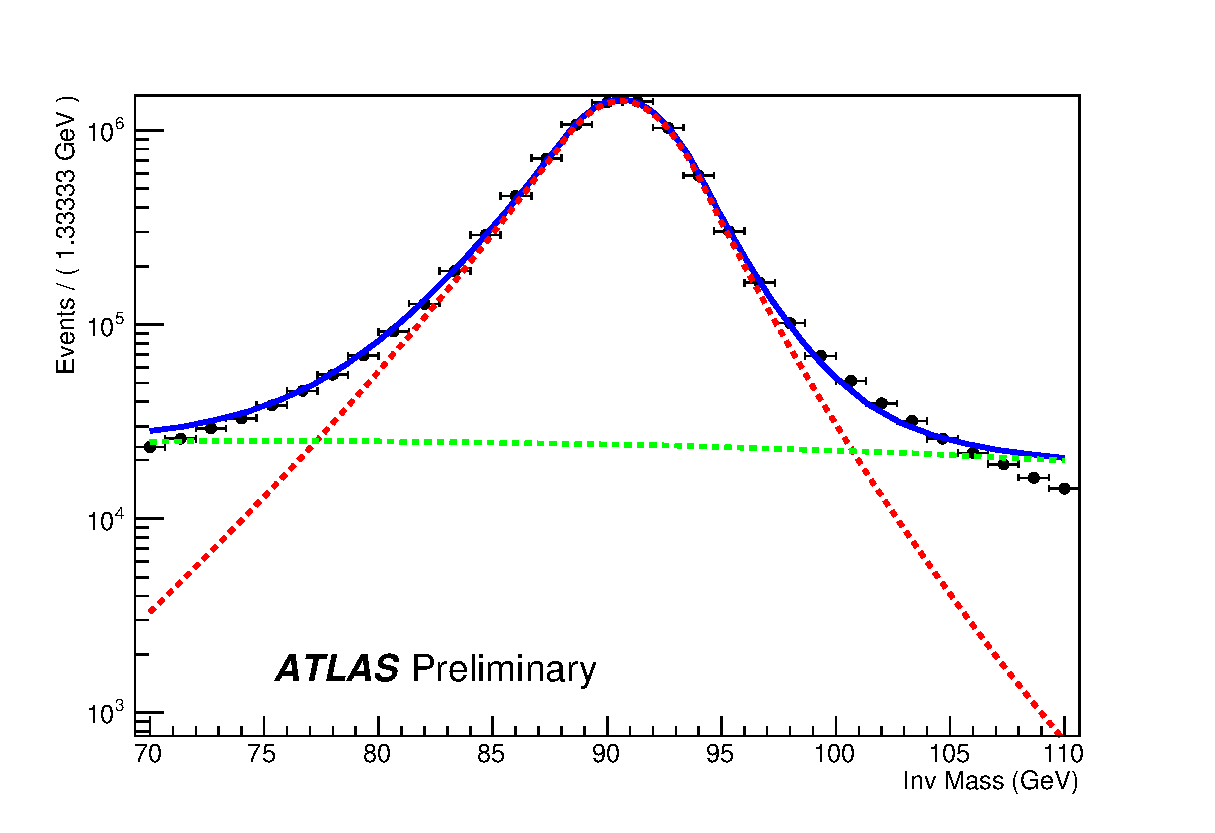
\includegraphics[scale=0.40]{d15_16_egam1_m_fit_h_m_ee_BB.eps} 
	\end{subfigure}
	~
	\begin{subfigure}{0.5\textwidth}
		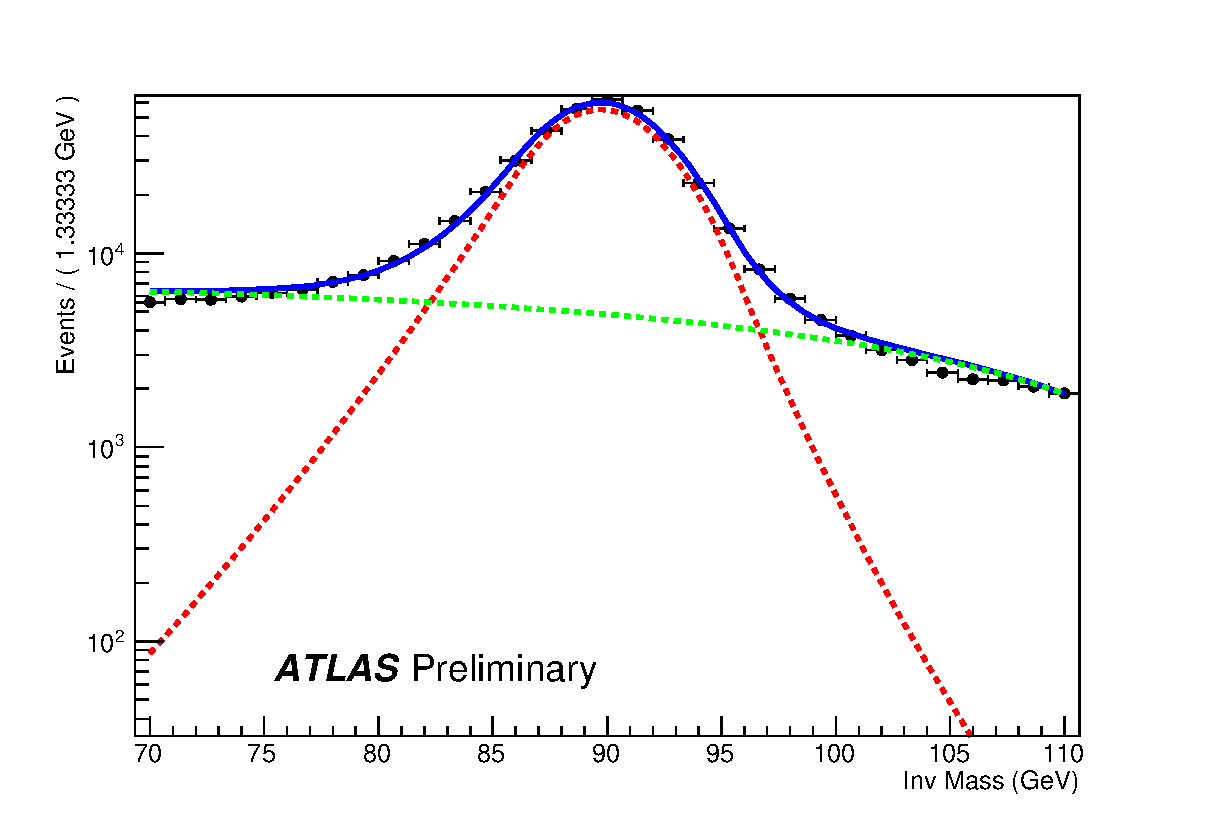
\includegraphics[scale=0.40]{d15_16_egam1_m_fit_h_m_eg_BB.eps}
	\end{subfigure}

	
	\caption{Fits de la masa invariante de los pares $ee$ (izquierda) y $e\gamma$ (derecha), reconstruidos en al región $BB$. La curva roja corresponde a la DSCB, la verde al polinomio de grado 2 y la azul a la combinación resultante de ambas.}
\label{fits_BB}
\end{figure}

\begin{figure}

	\begin{subfigure}{0.5\textwidth}
		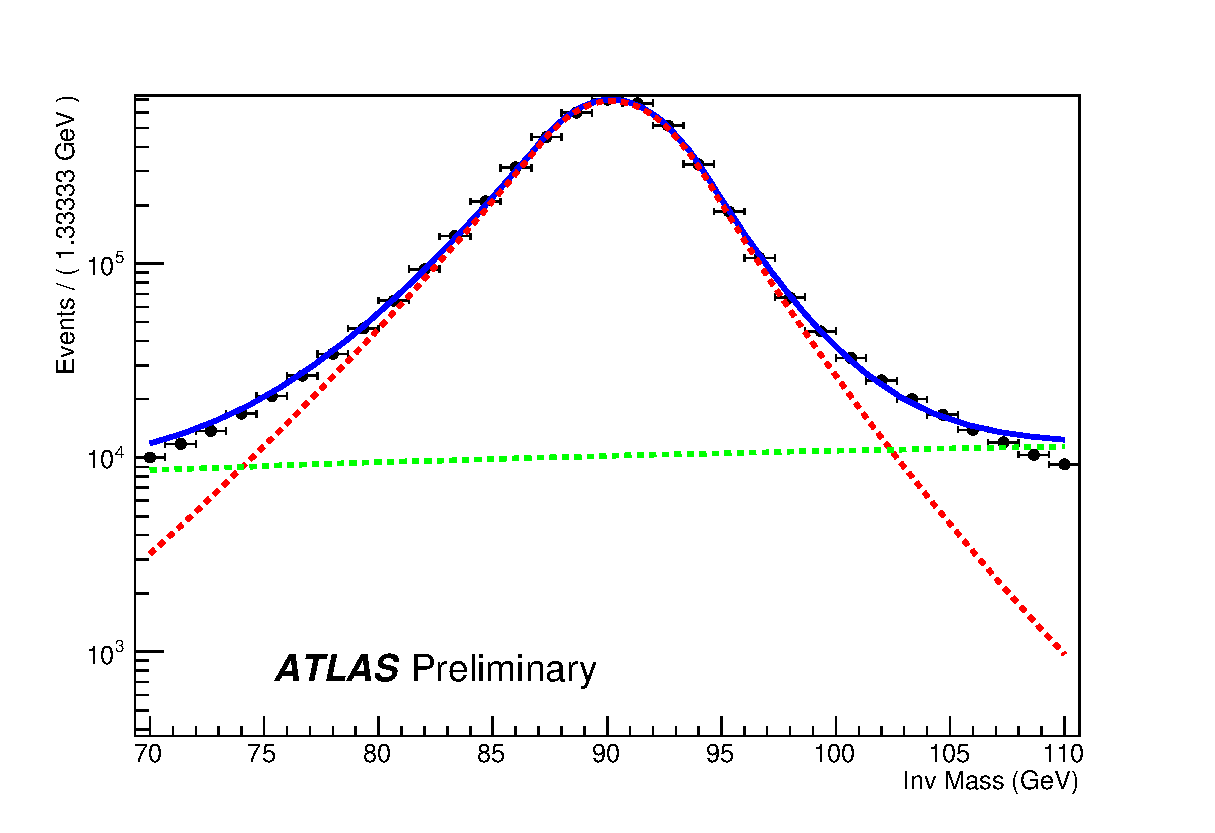
\includegraphics[scale=0.40]{d15_16_egam1_m_fit_h_m_ee_BE.eps} 
	\end{subfigure}
	~
	\begin{subfigure}{0.5\textwidth}
		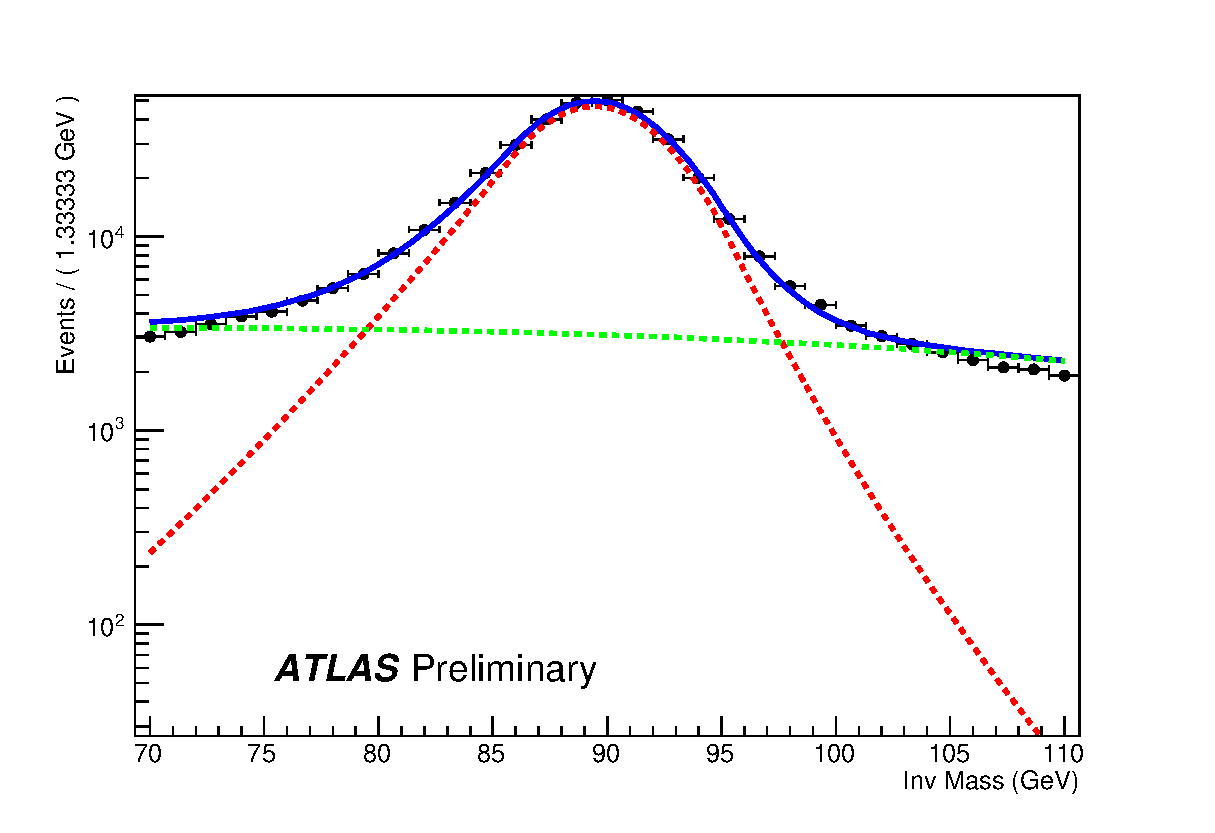
\includegraphics[scale=0.40]{d15_16_egam1_m_fit_h_m_eg_BE.eps}
	\end{subfigure}

	
	\caption{Fits de la masa invariante de los pares $ee$ (izquierda) y $e\gamma$ (derecha), reconstruidos en al región $BE$. La curva roja corresponde a la DSCB, la verde al polinomio de grado 2 y la azul a la combinación resultante de ambas.}
\label{fits_BE}
\end{figure}


\begin{figure}

	\begin{subfigure}{0.5\textwidth}
		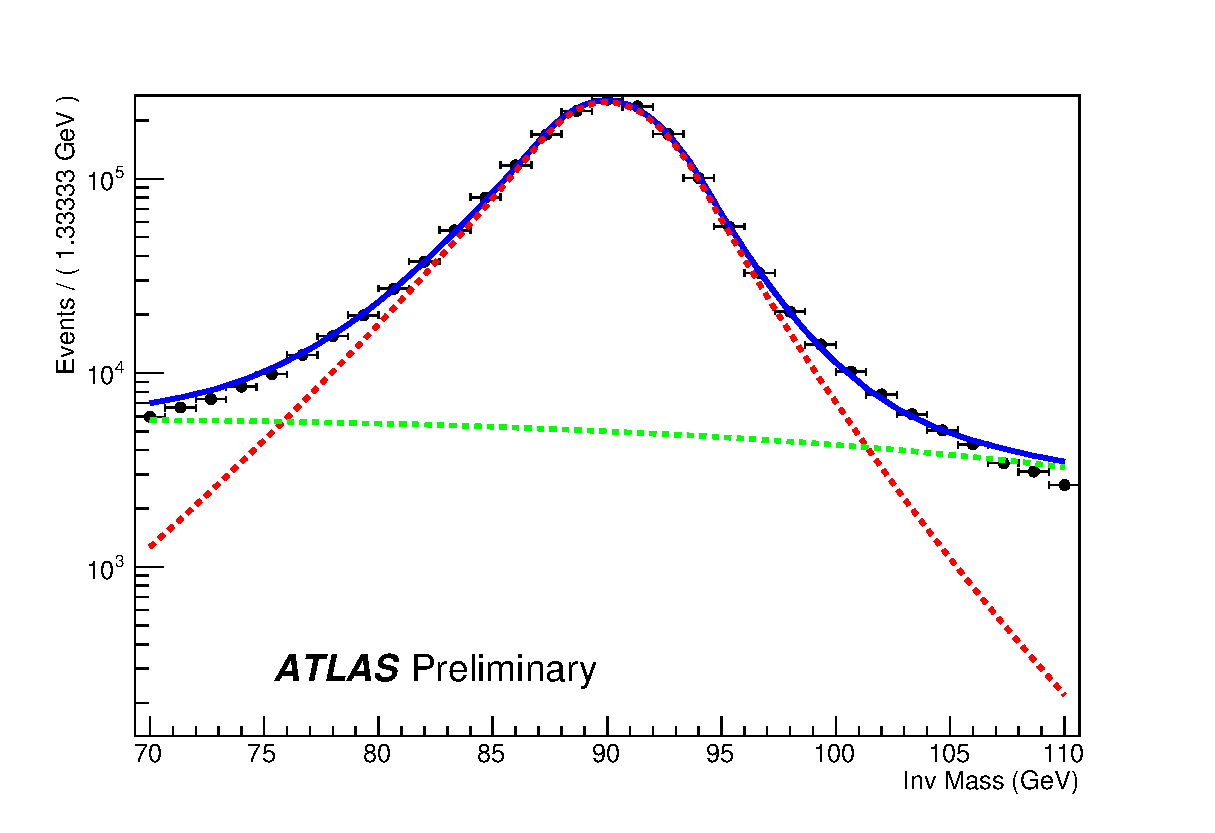
\includegraphics[scale=0.40]{d15_16_egam1_m_fit_h_m_ee_EE.eps} 
	\end{subfigure}
	~
	\begin{subfigure}{0.5\textwidth}
		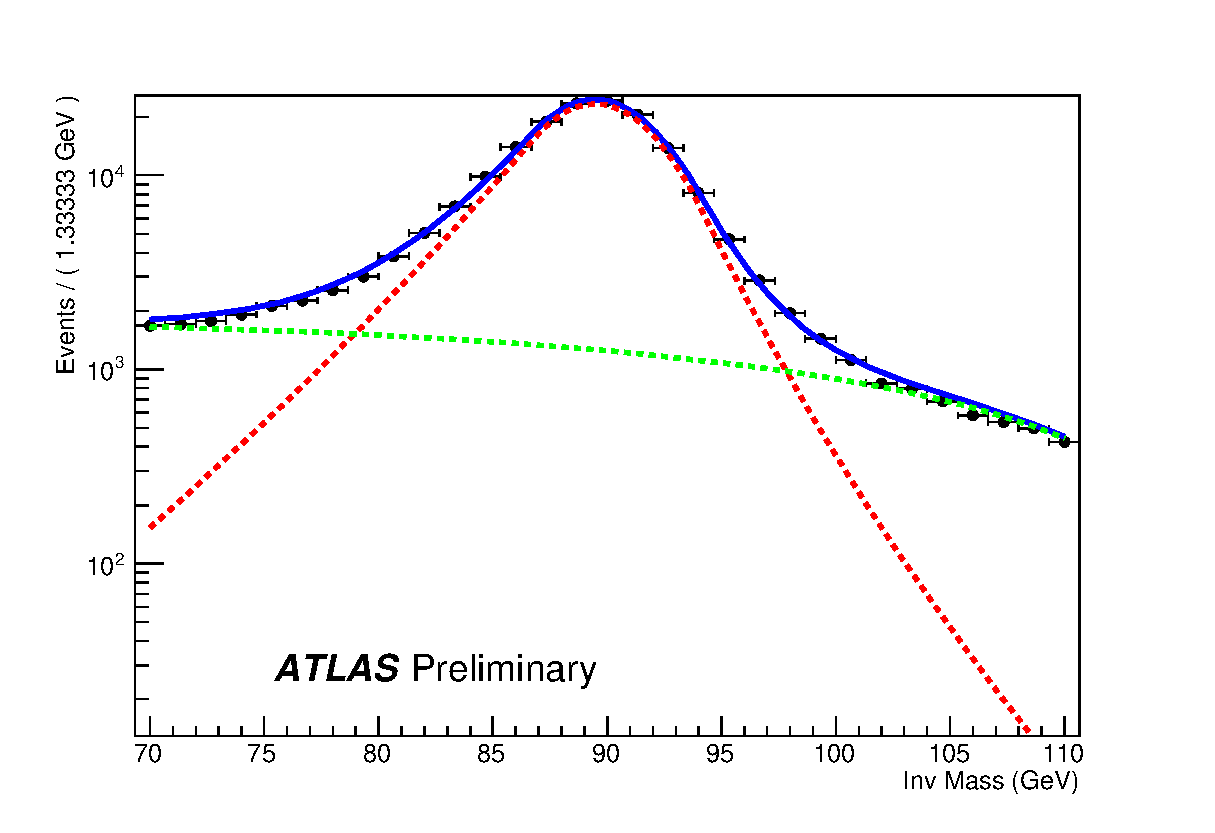
\includegraphics[scale=0.40]{d15_16_egam1_m_fit_h_m_eg_EE.eps}
	\end{subfigure}

	
	\caption{Fits de la masa invariante de los pares $ee$ (izquierda) y $e\gamma$ (derecha), reconstruidos en al región $EE$. La curva roja corresponde a la DSCB, la verde al polinomio de grado 2 y la azul a la combinación resultante de ambas.}
\label{fits_EE}
\end{figure}


\subsection{Resultados y estimación del fondo en regiones de control y validación} \label{sec:resultados}

\begin{table}	
\centering
\begin{threeparttable}
\caption{Tabla con los factores de identificación errónea en bines de $\eta$ y $p_{T}$, con sus valores de incerteza estadística y sistemática.}
\begin{tabular}{ l l c c c c c c }

	\hline
	\hline

	\multirow{2}{*}{$|\eta|$} & \multirow{2}{*}{$p_{T}$[GeV]} & \multirow{2}{*}{Fake factor} & \multirow{2}{*}{Estad.} & \multicolumn{4}{c}{Sistemáticos} \\

	\cline{5-8}

	 & & & & Bern 4$\degree$ & Poli 3$\degree$ & Rango & Total \\


	\hline

	0 - 0.6 & 75 - 90 & 0.0168 & 0.0003 & -			& 0.0003  &  0.0004 &  0.0006  \\

	0 - 0.6 & 90 - 145 & 0.0158 & 0.0004 & - 		& 0.0002  &  0.0003 &  0.0005  \\

	0 - 0.6 & 145 - 300 & 0.0142 & 0.0007 & -  		& 0.0002  &  0.0003 &  0.0008  \\

	\hline

	0.6 - 1.37 & 75 - 90 & 0.0186 & 0.0003 & -		& 0.0002  &  0.0004 &  0.0005  \\

	0.6 - 1.37 & 90 - 145 & 0.0183 & 0.0004 & -		& 0.0002  &  0.0004 &  0.0006  \\

	0.6 - 1.37 & 145 - 300 & 0.0141 & 0.0007 & -  	& 0.0002  &  0.0003 &  0.0008  \\

	\hline

	1.52 - 1.82 & 75 - 90 & 0.0354  & 0.0009 & -		& 0.0003  &  0.001 &  0.001  \\

	1.52 - 1.82 & 90 - 145 & 0.033  & 0.001 & -		& 0.001  &  0.001  &  0.002 \\

	1.52 - 1.82 & 145 - 300 & 0.026  & 0.002 & -  	& 0  &  0.0005  &  0.002  \\

	\hline

	1.82 - 2.37 & 75 - 90 & 0.045  & 0.001 & -		& 0.0001  &  0.001 &  0.001  \\

	1.82 - 2.37 & 90 - 145 & 0.040  & 0.001 & -		& 0.001  &  0.002  &  0.002  \\

	1.82 - 2.37 & 145 - 300 & 0.038  & 0.002 & -  	& 0  &  0.002  &  0.003  \\

	\hline
	\hline

\end{tabular}
\label{ta:fftable}
\end{threeparttable}
\end{table}


Observando los resultados expuestos en las distintas tablas, definimos la implementación de una selección \textit{medium} de los electrones ya que los valores de pureza (expresado en los valores de los pesos $w$) e incertezas sistemáticas son equivalentes a la selección \textit{tight}, pero con la ventaja de una mayor estadística de eventos para estimar el fondo en las distintas regiones de control y validación.


\tosolve{Acá van los gráficos de Fran de las regiones de control y validación.}
